\problemname{Klompendans}

\newcommand{\maxn}{500}

In traditional Dutch clog dancing, you as the dancer need to follow a very specific sequence of movements.
The dance takes place on a square grid of square tiles, and at the start of the dance you stand on the top left corner tile of the grid.
You then alternate between two types of dance move, moving from tile to tile in the grid for as long as you want.
Your first move may be of either kind, but after that you need to strictly alternate between the two kinds of moves.

Both moves are similar to knight moves in chess:
in the first type of move, you go from your current square to a square that is $a$ tiles away along one axis of the grid and $b$ tiles away along the other axis.
Similarly, in the second type of move, you need to move $c$ and $d$ tiles along the respective axes.
As you can freely swap the two axes and choose the movement direction along each axis, there can be up to $8$ ways of performing a given type of move.
Figure~\ref{fig:clogdance} shows an example dance routine with $(a,b) = (1,2)$ and $(c,d) = (2,3)$.

\begin{figure}[!h]
  \centering
  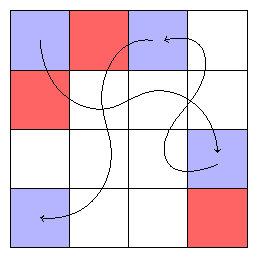
\includegraphics[width=0.4\textwidth]{figure}
  \caption{
    Illustration of Sample Input 3, showing a dance that begins in the top left corner of a $4\times 4$ grid and ends in the bottom left corner, visiting the blue squares along the way.
    There are $13$ reachable squares in total.
    The three squares highlighted in red cannot be part of any dance performance.
  }
  \label{fig:clogdance}
\end{figure}

Starting on the top left corner tile, how many different tiles could you reach while doing a clog dance?
It is not allowed to step outside of the grid and you do not count tiles that you are simply stepping over while doing a move.
Note that you need to count all tiles that can be reached during \emph{some} performance of the dance, but not necessarily during the same one.

\begin{Input}
  The input consists of:
  \begin{itemize}
    \item One line with an integer $n$ ($3\leq n\leq \maxn$), the side length of the square.
    \item One line with two integers $a$ and $b$ ($1\leq a, b < n$), describing the first dance move.
    \item One line with two integers $c$ and $d$ ($1\leq c, d < n$), describing the second dance move.
  \end{itemize}
\end{Input}

\begin{Output}
  Output the number of tiles you can reach using these dance moves.
\end{Output}
